
The following figures show the array factor patterns for a 5x5 planar antenna array with different spacings ($d$) and steering angles (either vertical or $\theta_{d}=60\,\si{\degree}$), calculated with python. The array geometry can be seen in figure \ref{fig:phase1}.\\

One can see grating lobes appear on the edges of some radiation patterns due to the finite antenna distances involved. As the distance between the antennas goes down, the angular distance towards the grating lobes increases, i.e. angular ambiguities appear ``later'' and the beam can be safely steered to greater angles. However, this also results in a greater beamwidth which might not be desired.\\

\begin{figure}[H]
  \begin{minipage}[t]{0.45\textwidth}
    \centering
    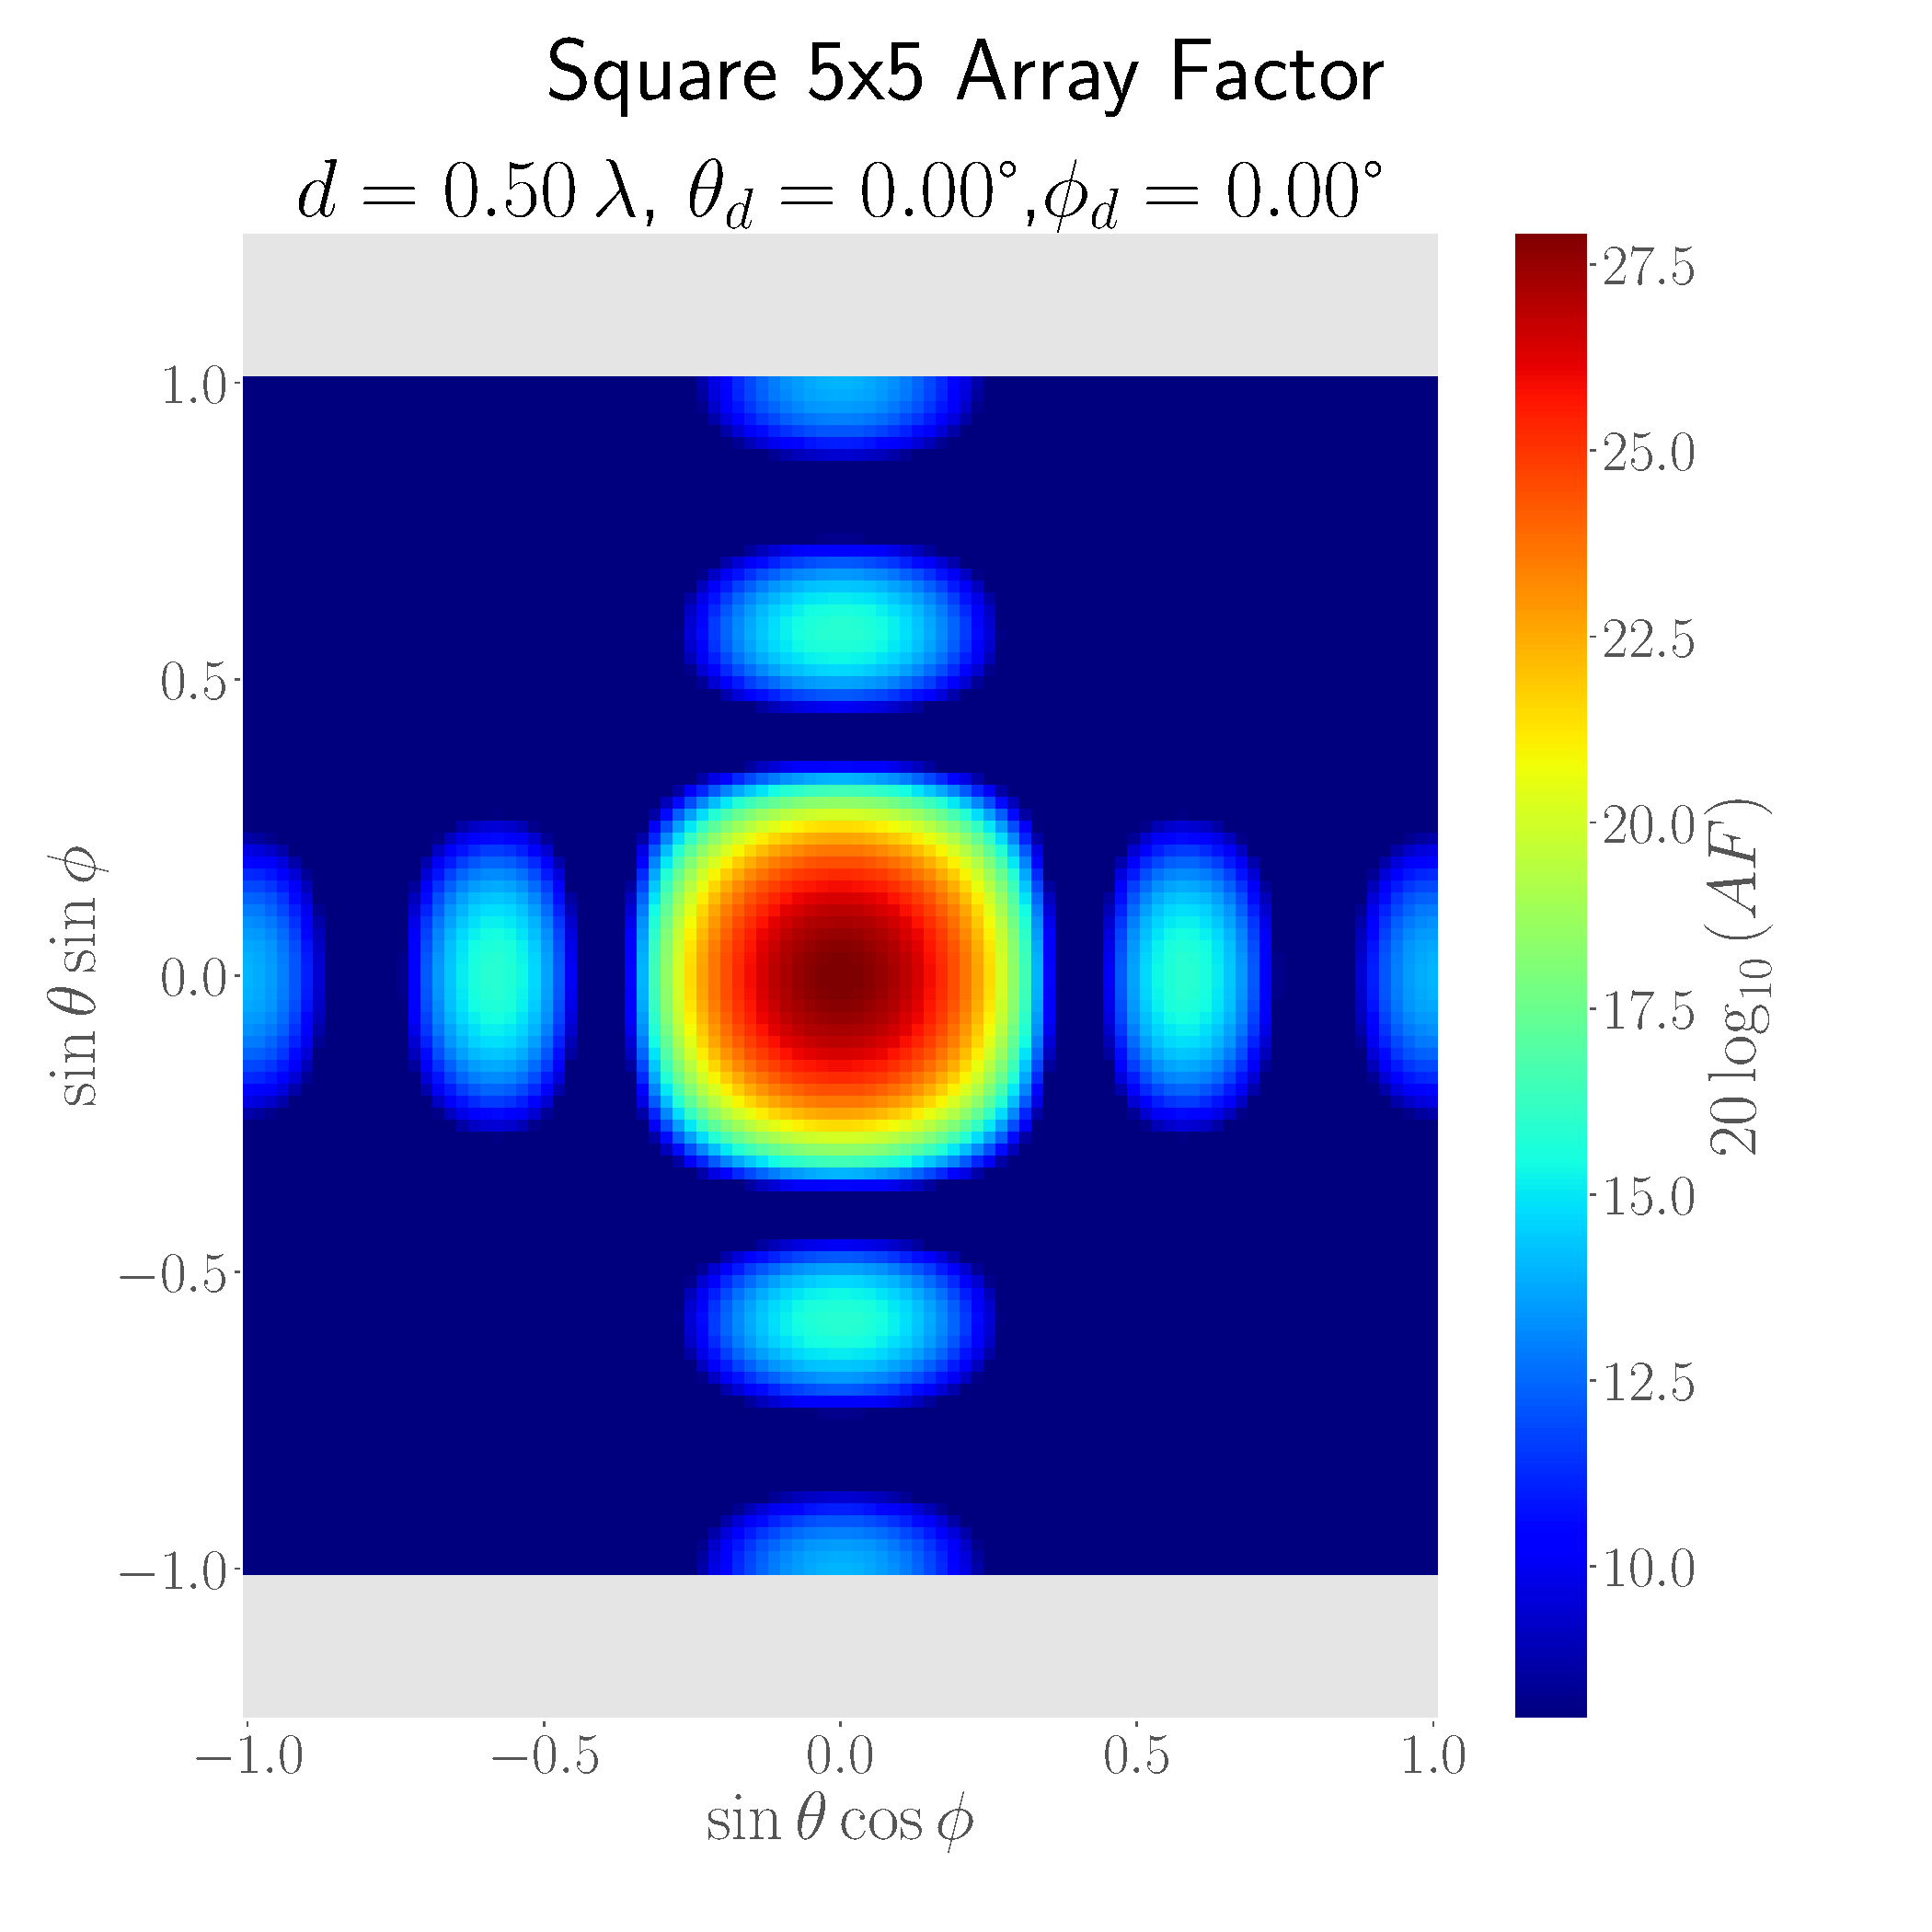
\includegraphics[width=\textwidth]{graphics/task_1/square-0.50-lambda-0.00-theta-0.00-phi-radpat.pdf}
    \caption{Square 5x5 vertically steered radiation pattern for $0.5\lambda$ spacing.}\label{fig:rad-square-0.5-0}
  \end{minipage}\hfill
  \begin{minipage}[t]{0.45\textwidth}
    \centering
    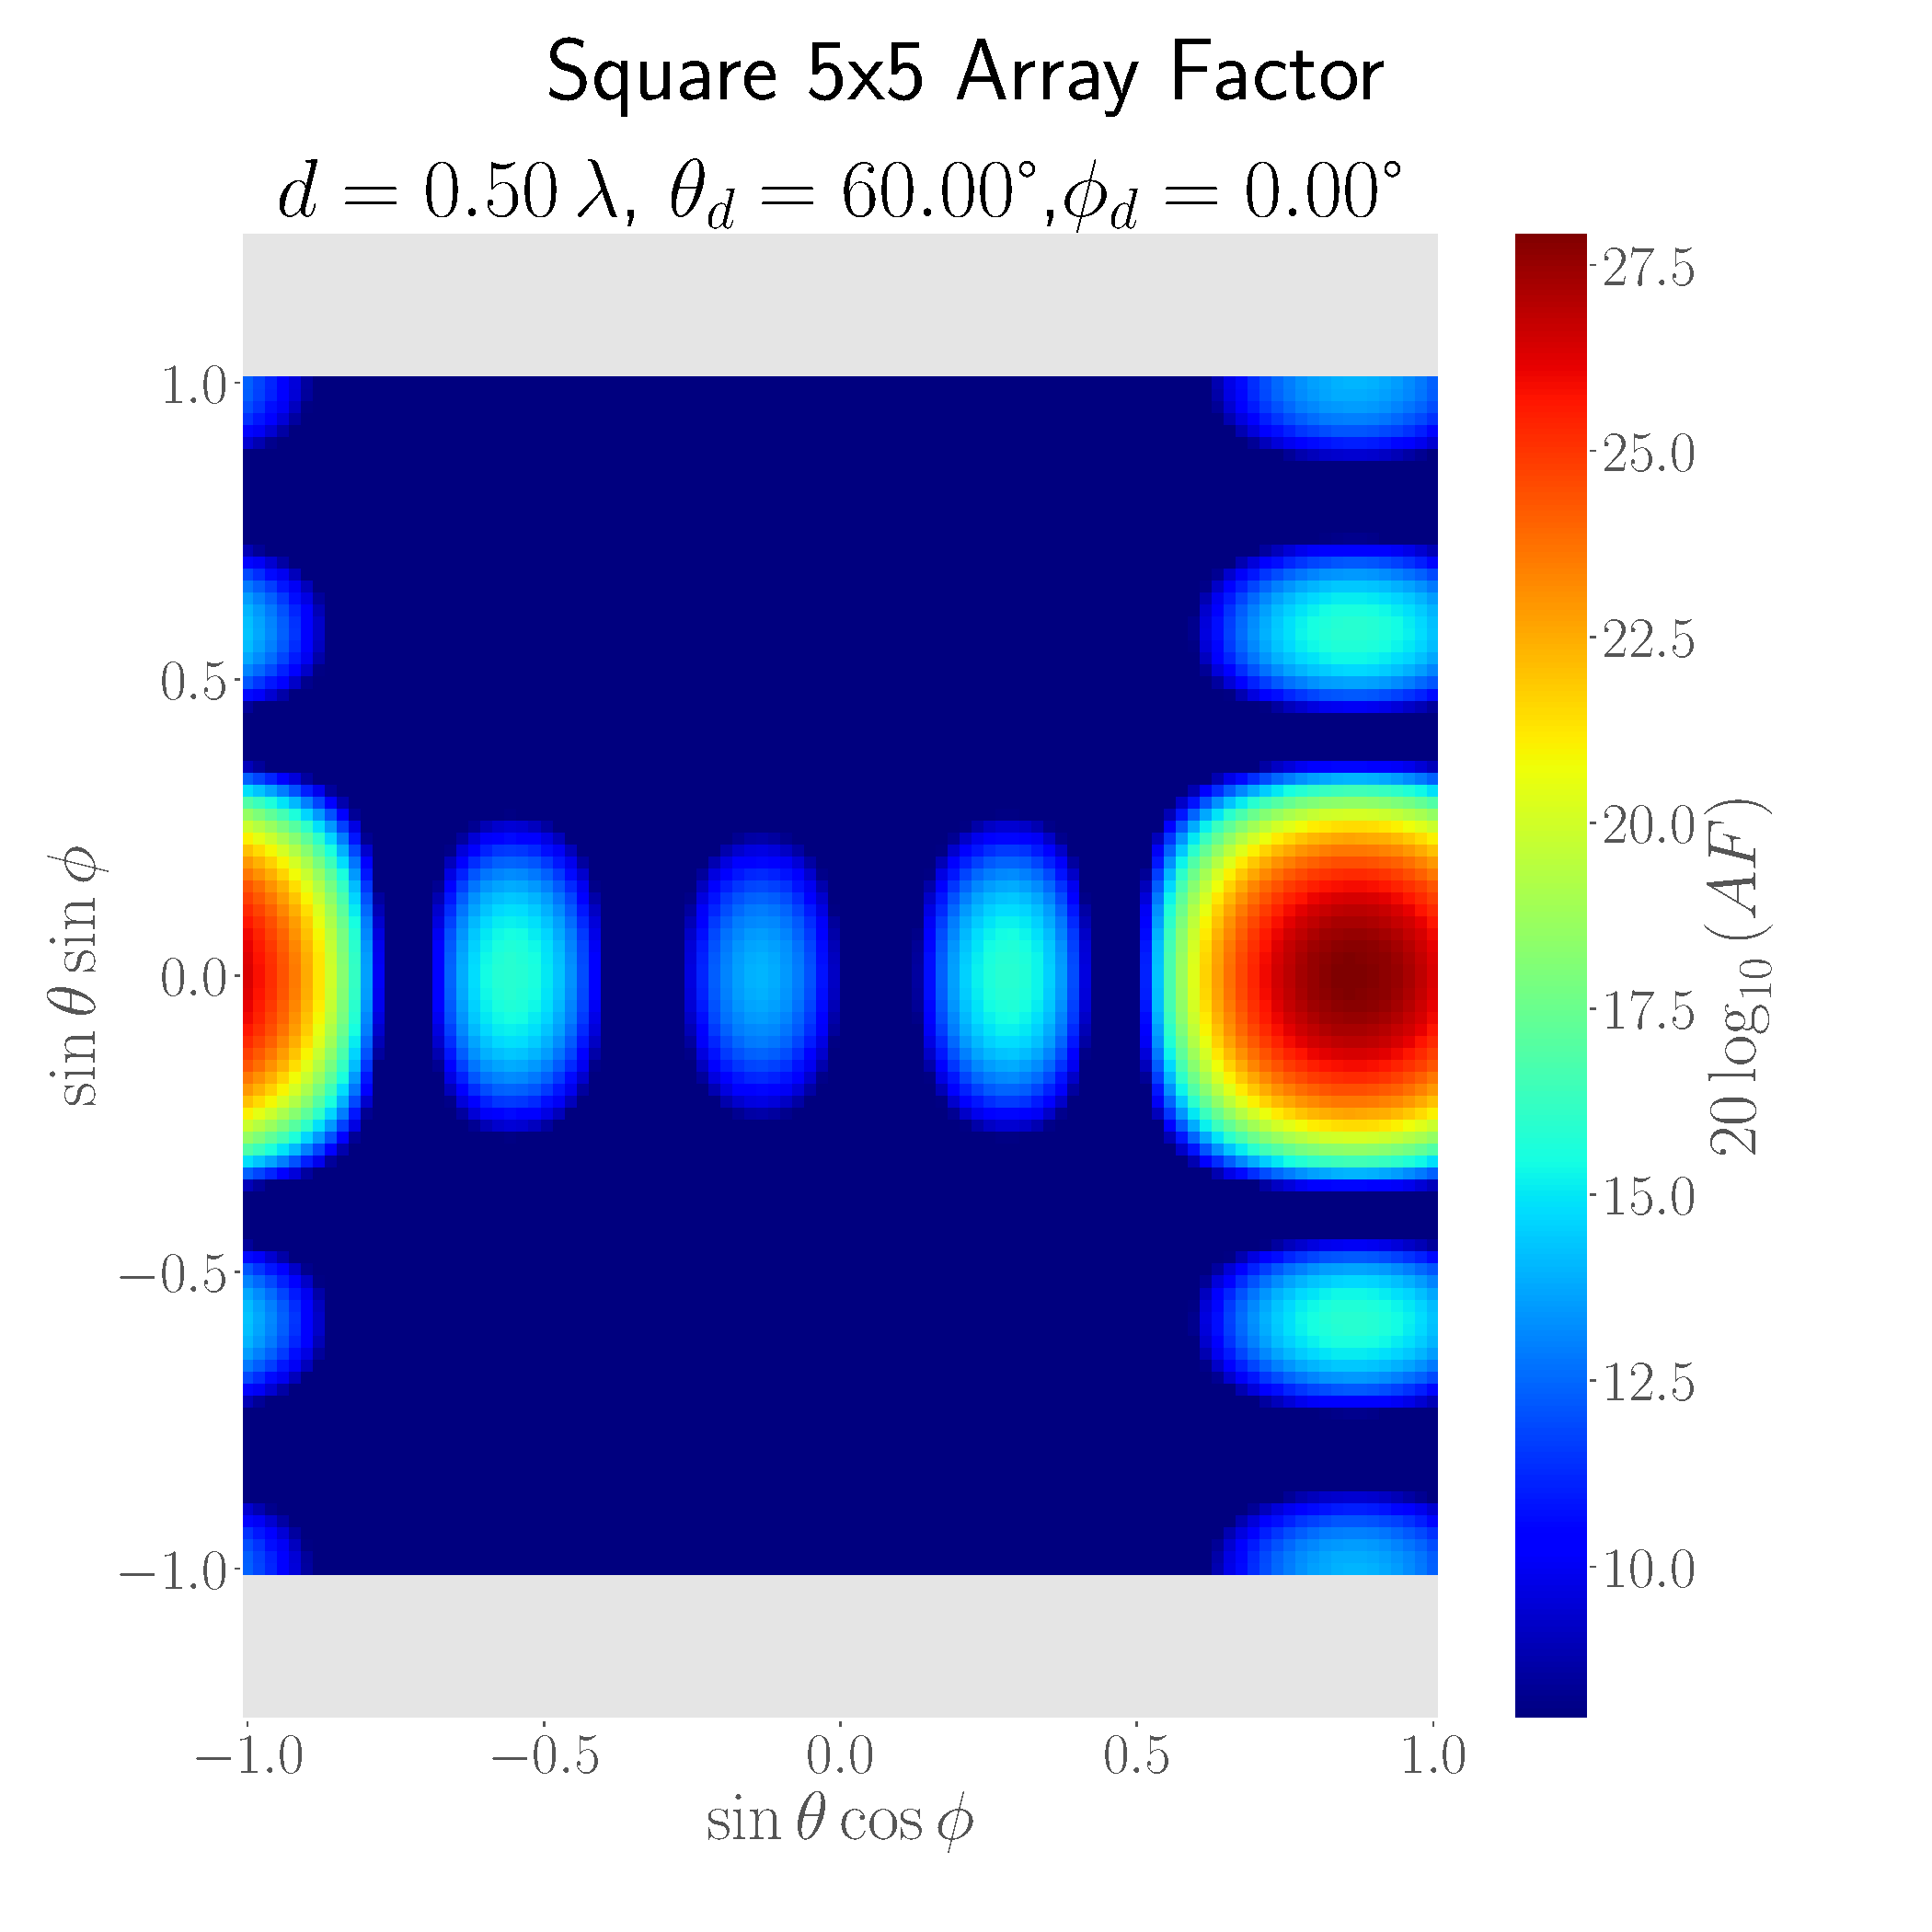
\includegraphics[width=\textwidth]{graphics/task_1/square-0.50-lambda-60.00-theta-0.00-phi-radpat.pdf}
    \caption{Square 5x5 off-vertically steered radiation pattern for $0.5\lambda$ spacing.}\label{fig:rad-square-0.5-60}
   \end{minipage}
\end{figure}

\begin{figure}[H]
  \begin{minipage}[t]{0.45\textwidth}
    \centering
    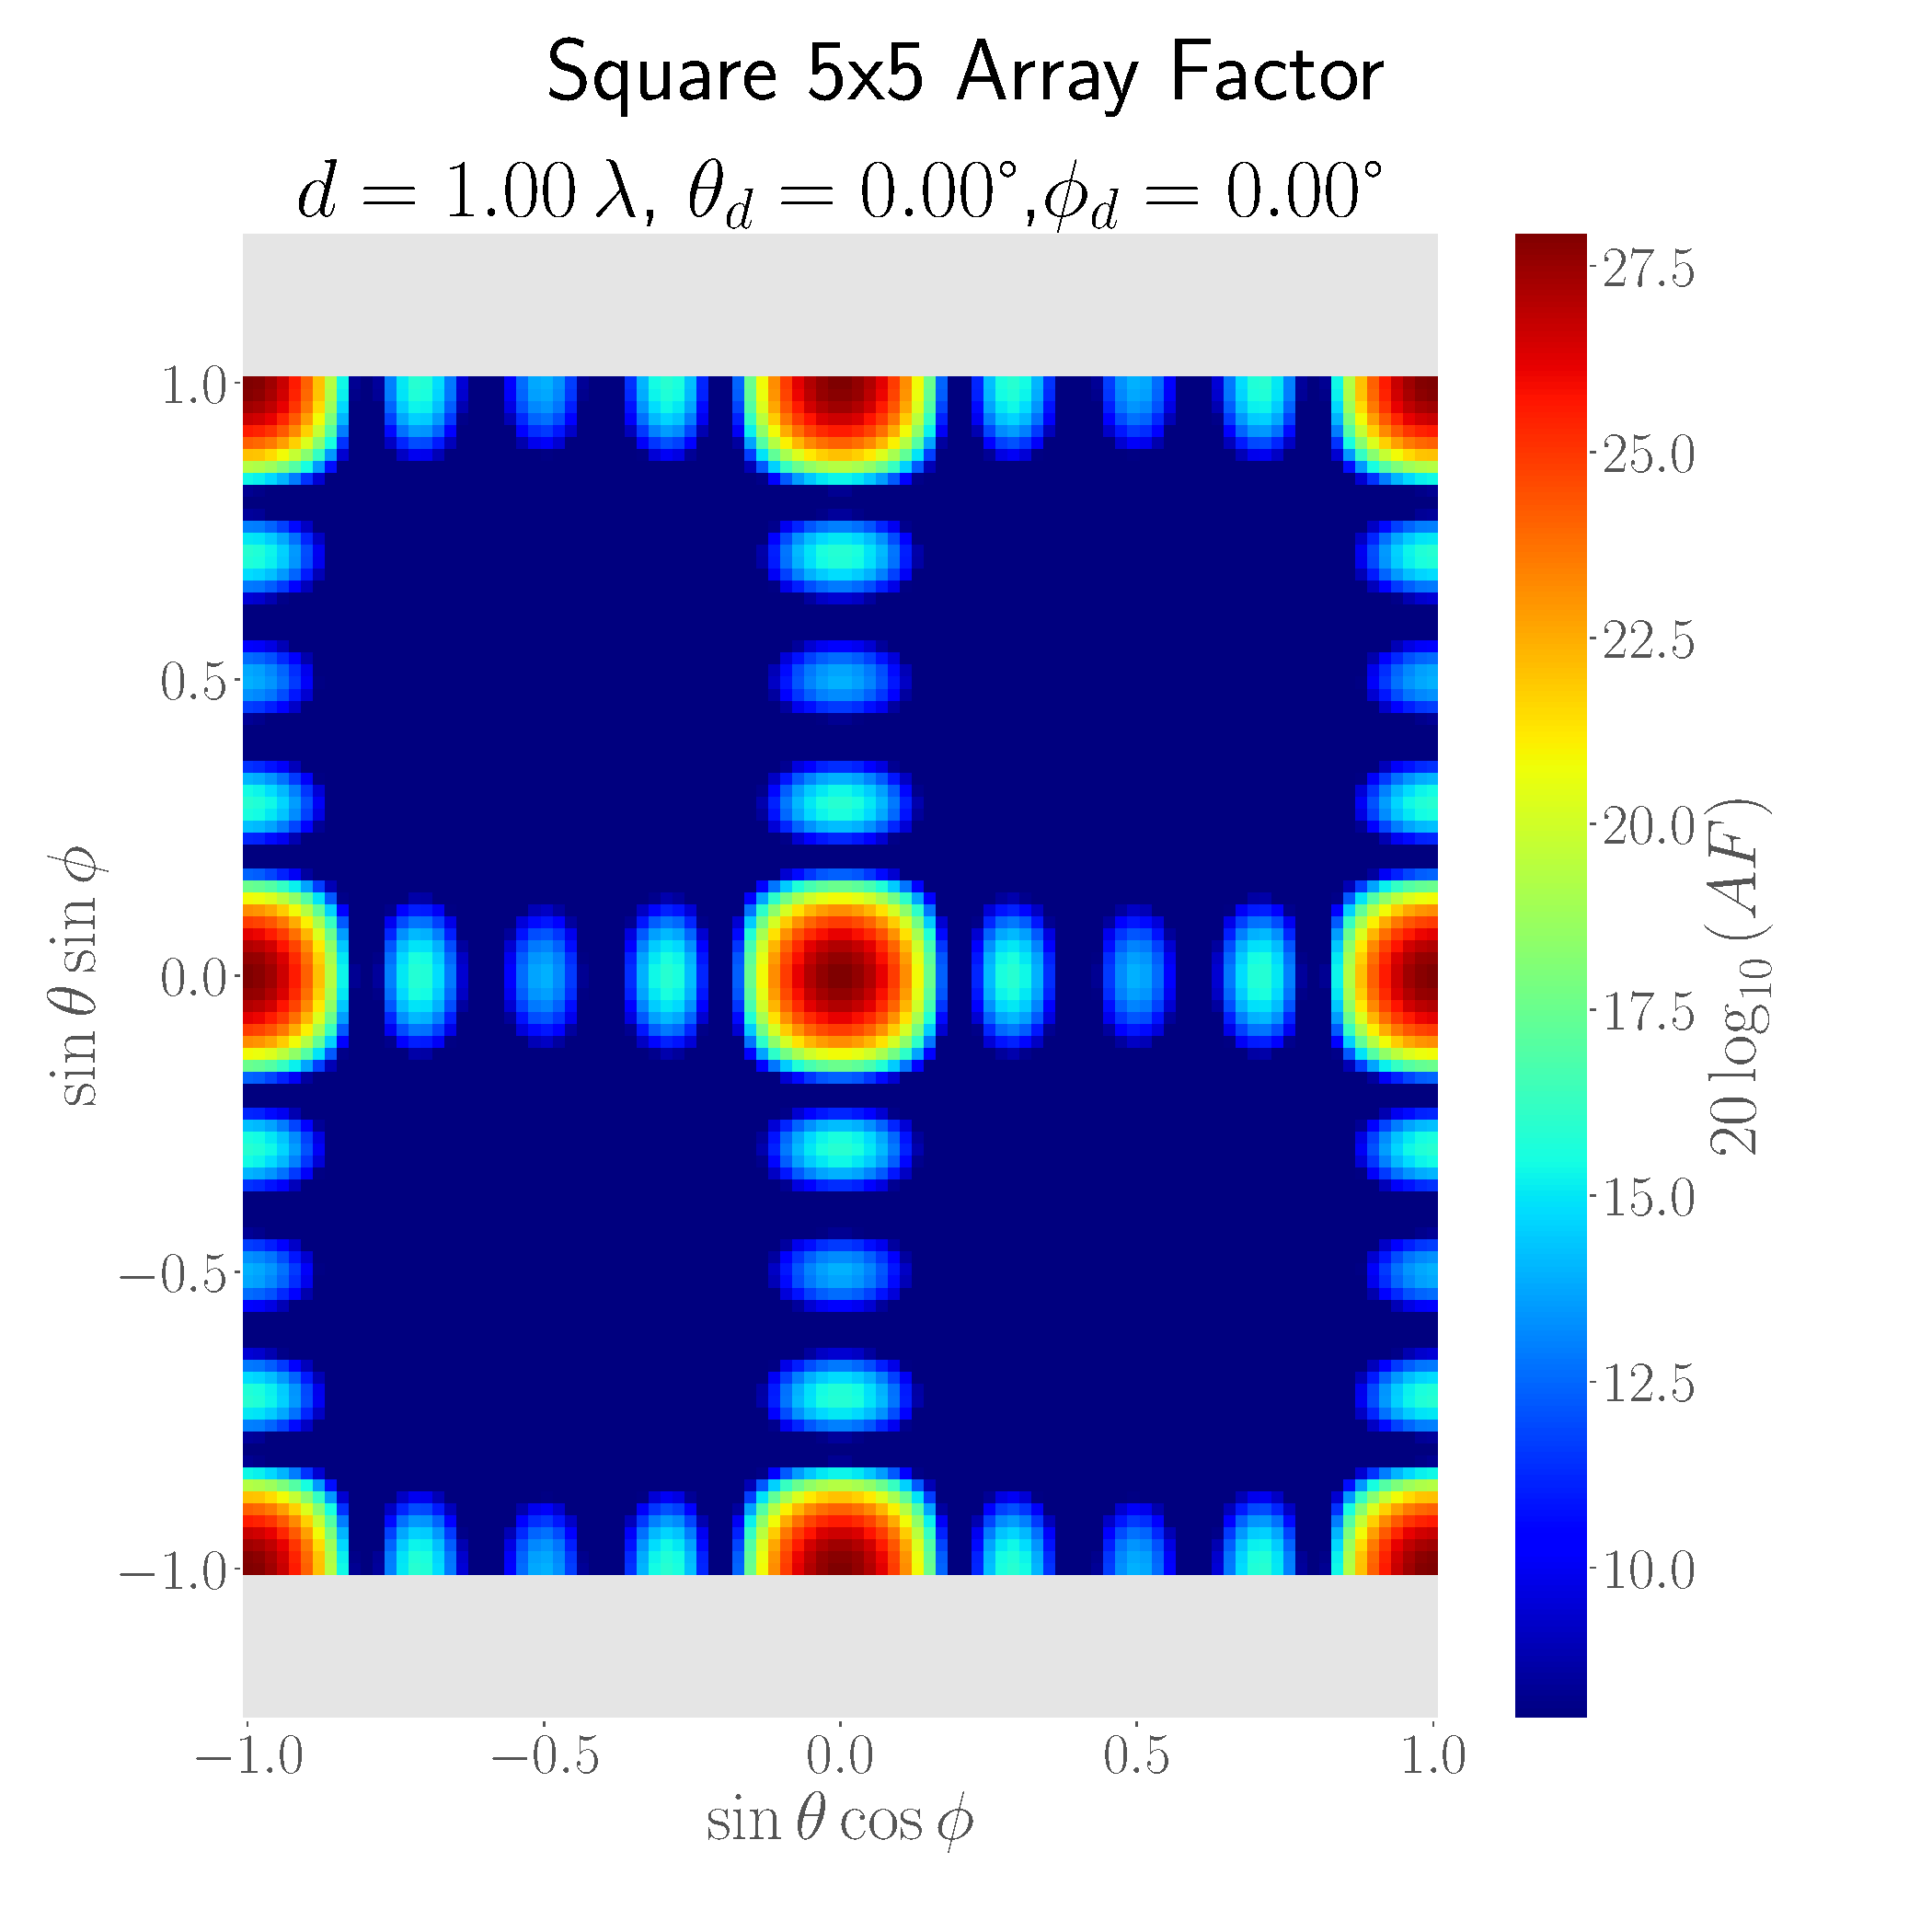
\includegraphics[width=\textwidth]{graphics/task_1/square-1.00-lambda-0.00-theta-0.00-phi-radpat.pdf}
    \caption{Square 5x5 vertically steered radiation pattern for $1.0\lambda$ spacing.}\label{fig:rad-square-1.0-0}
  \end{minipage}\hfill
  \begin{minipage}[t]{0.45\textwidth}
    \centering
    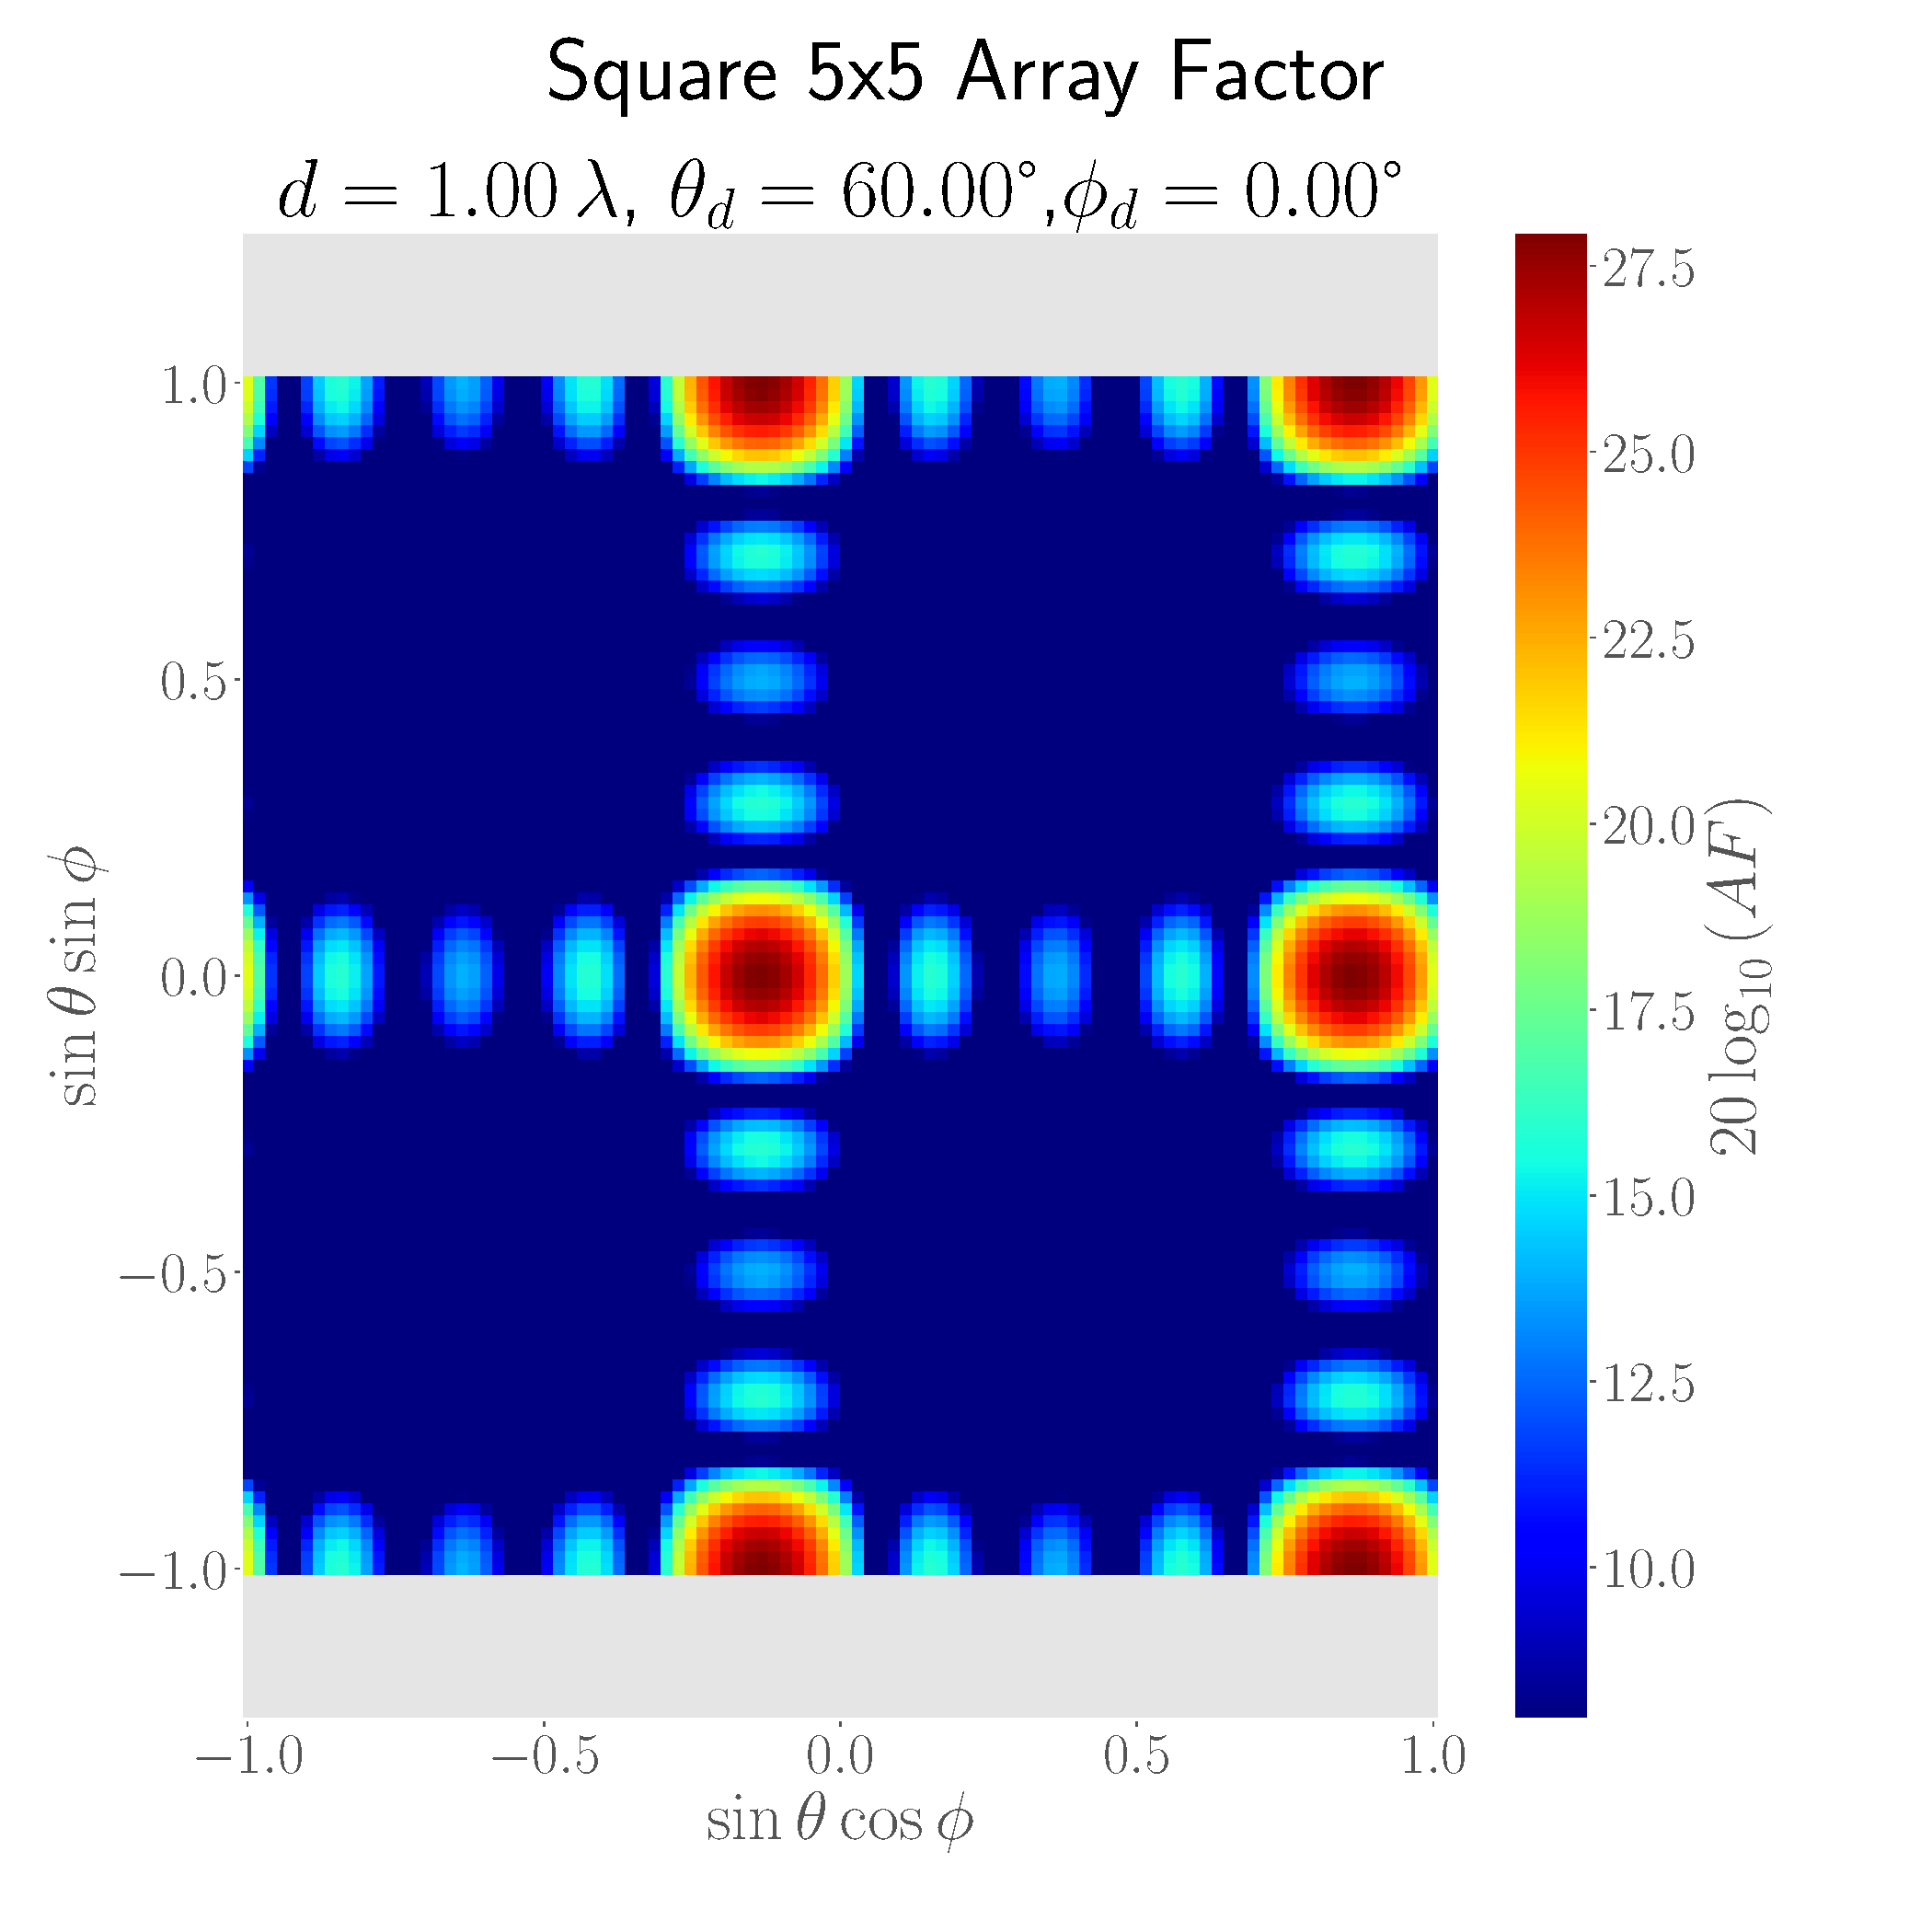
\includegraphics[width=\textwidth]{graphics/task_1/square-1.00-lambda-60.00-theta-0.00-phi-radpat.pdf}
    \caption{Square 5x5 off-vertically steered radiation pattern for $1.0\lambda$ spacing.}\label{fig:rad-square-1.0-60}
   \end{minipage}
\end{figure}

\begin{figure}[H]
  \begin{minipage}[t]{0.45\textwidth}
    \centering
    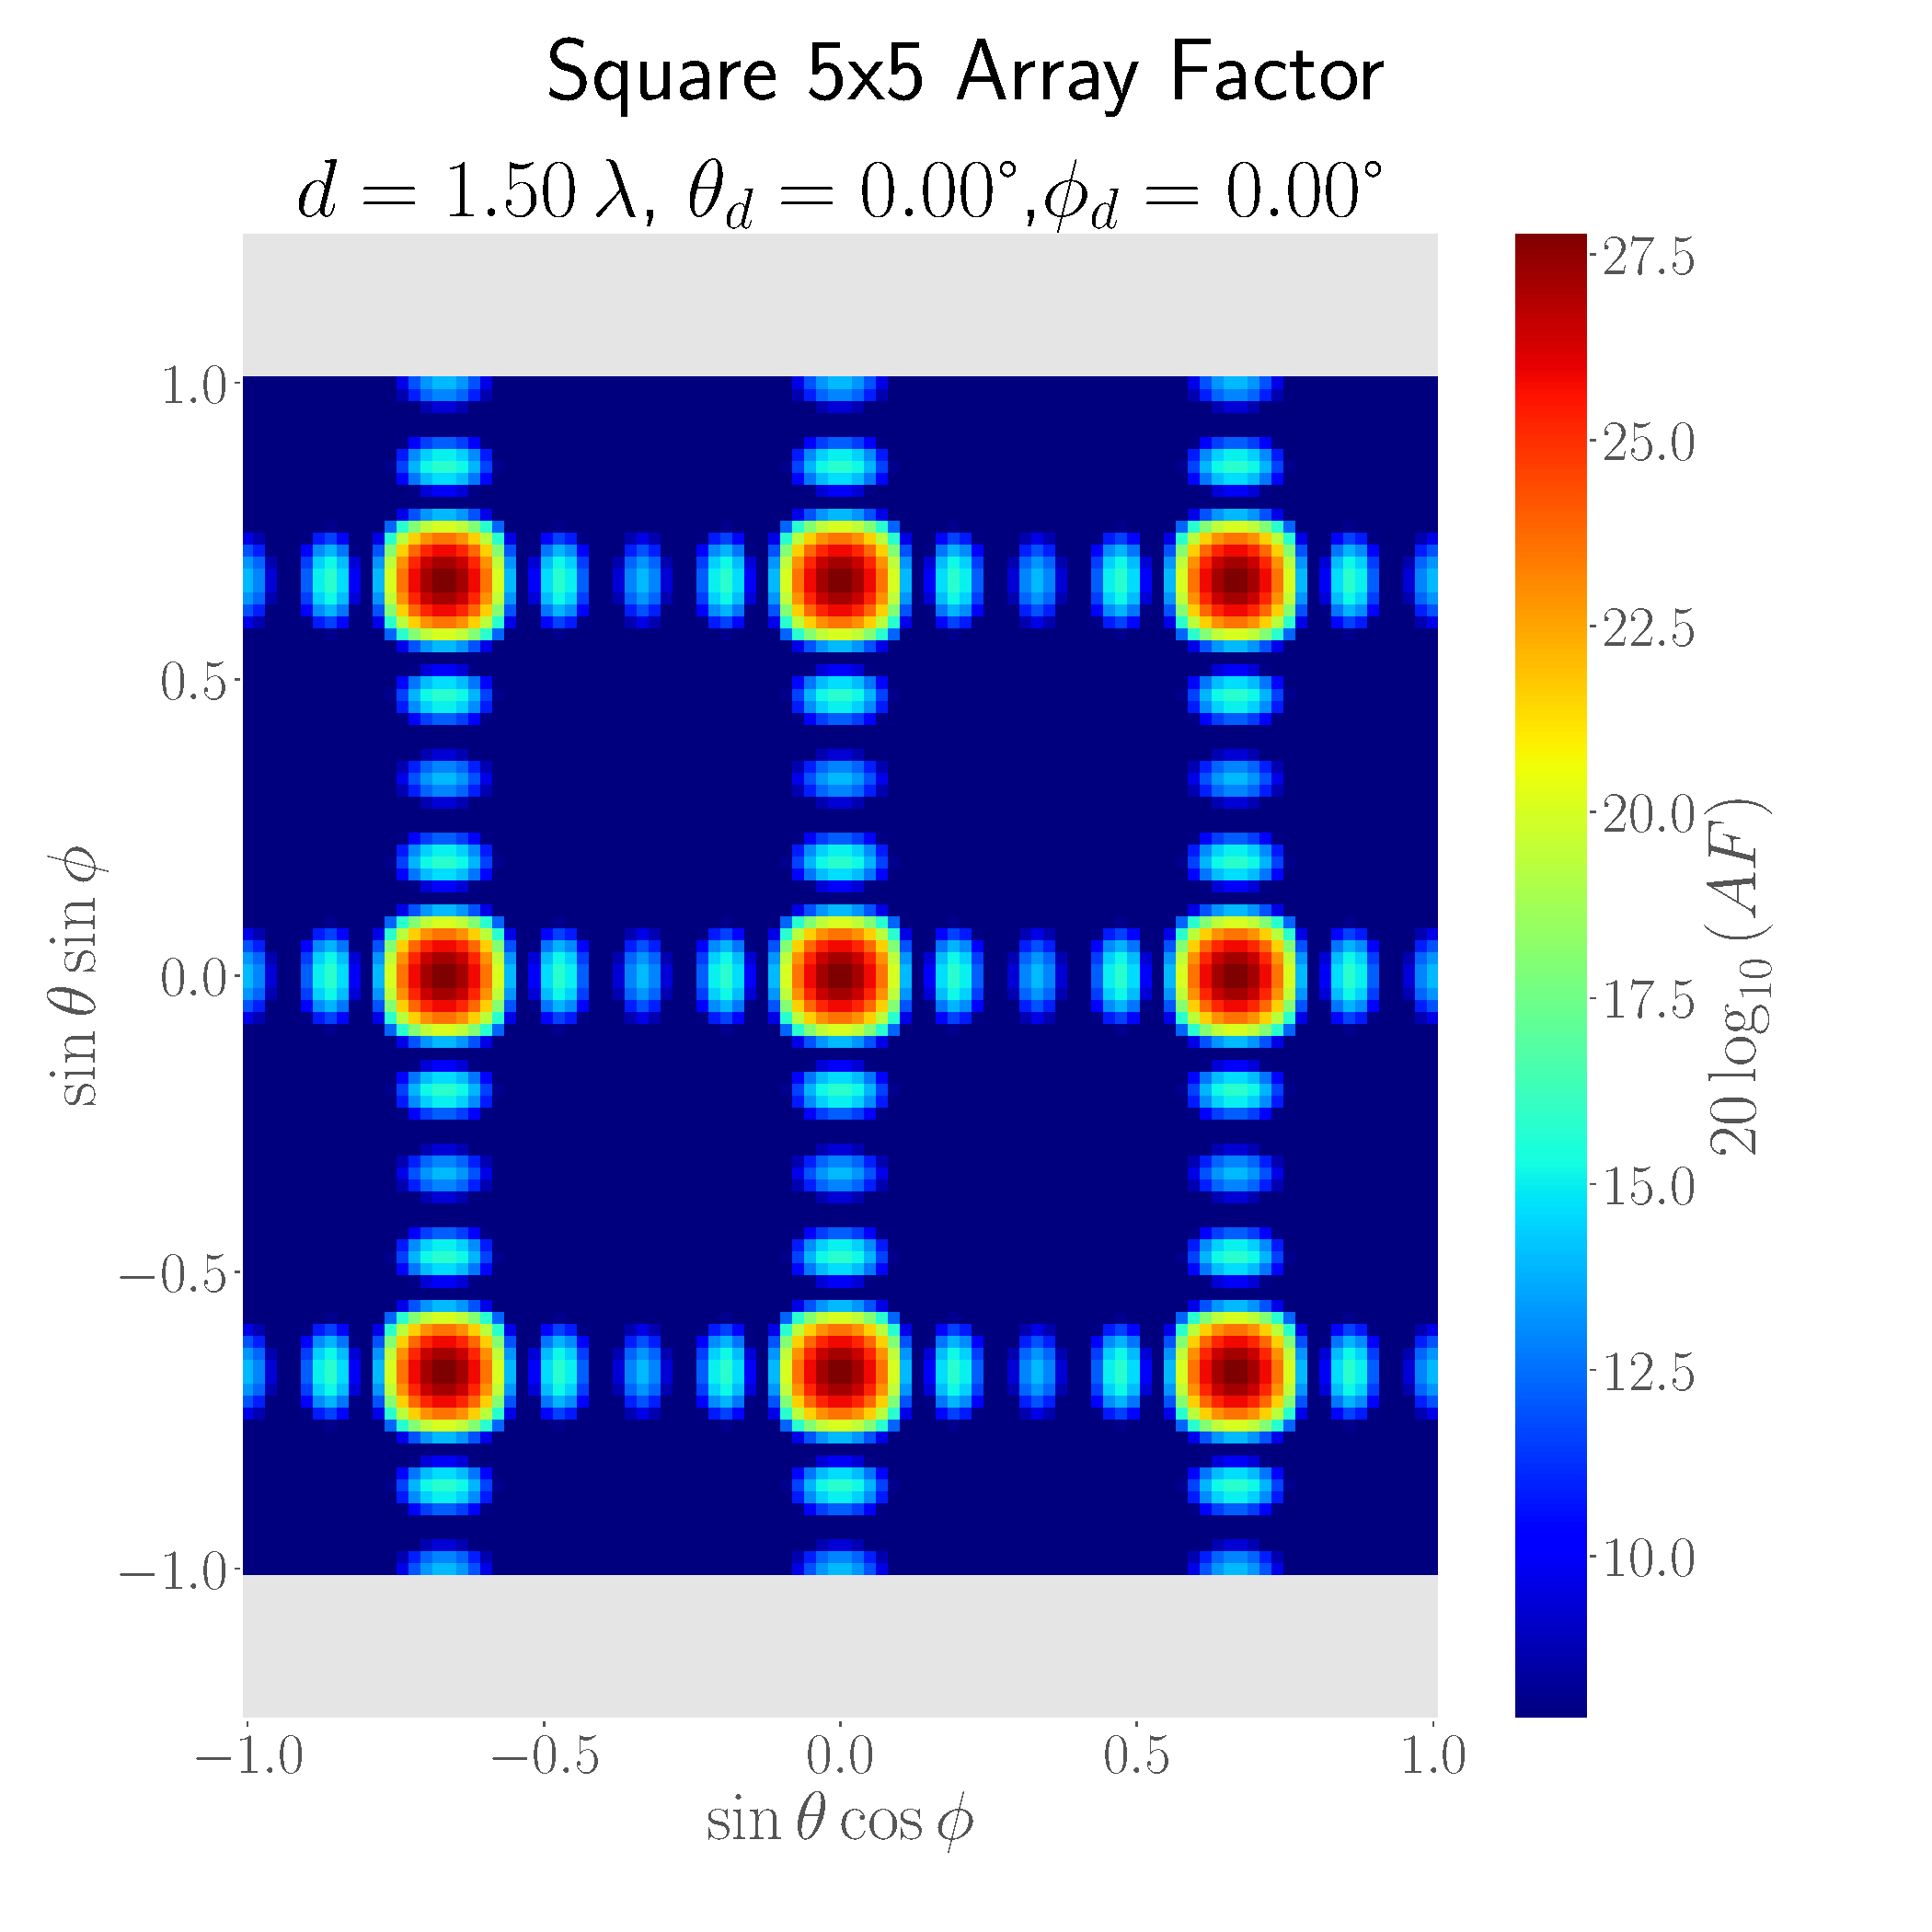
\includegraphics[width=\textwidth]{graphics/task_1/square-1.50-lambda-0.00-theta-0.00-phi-radpat.pdf}
    \caption{Square 5x5 vertically steered radiation pattern for $1.5\lambda$ spacing.}\label{fig:rad-square-1.5-0}
  \end{minipage}\hfill
  \begin{minipage}[t]{0.45\textwidth}
    \centering
    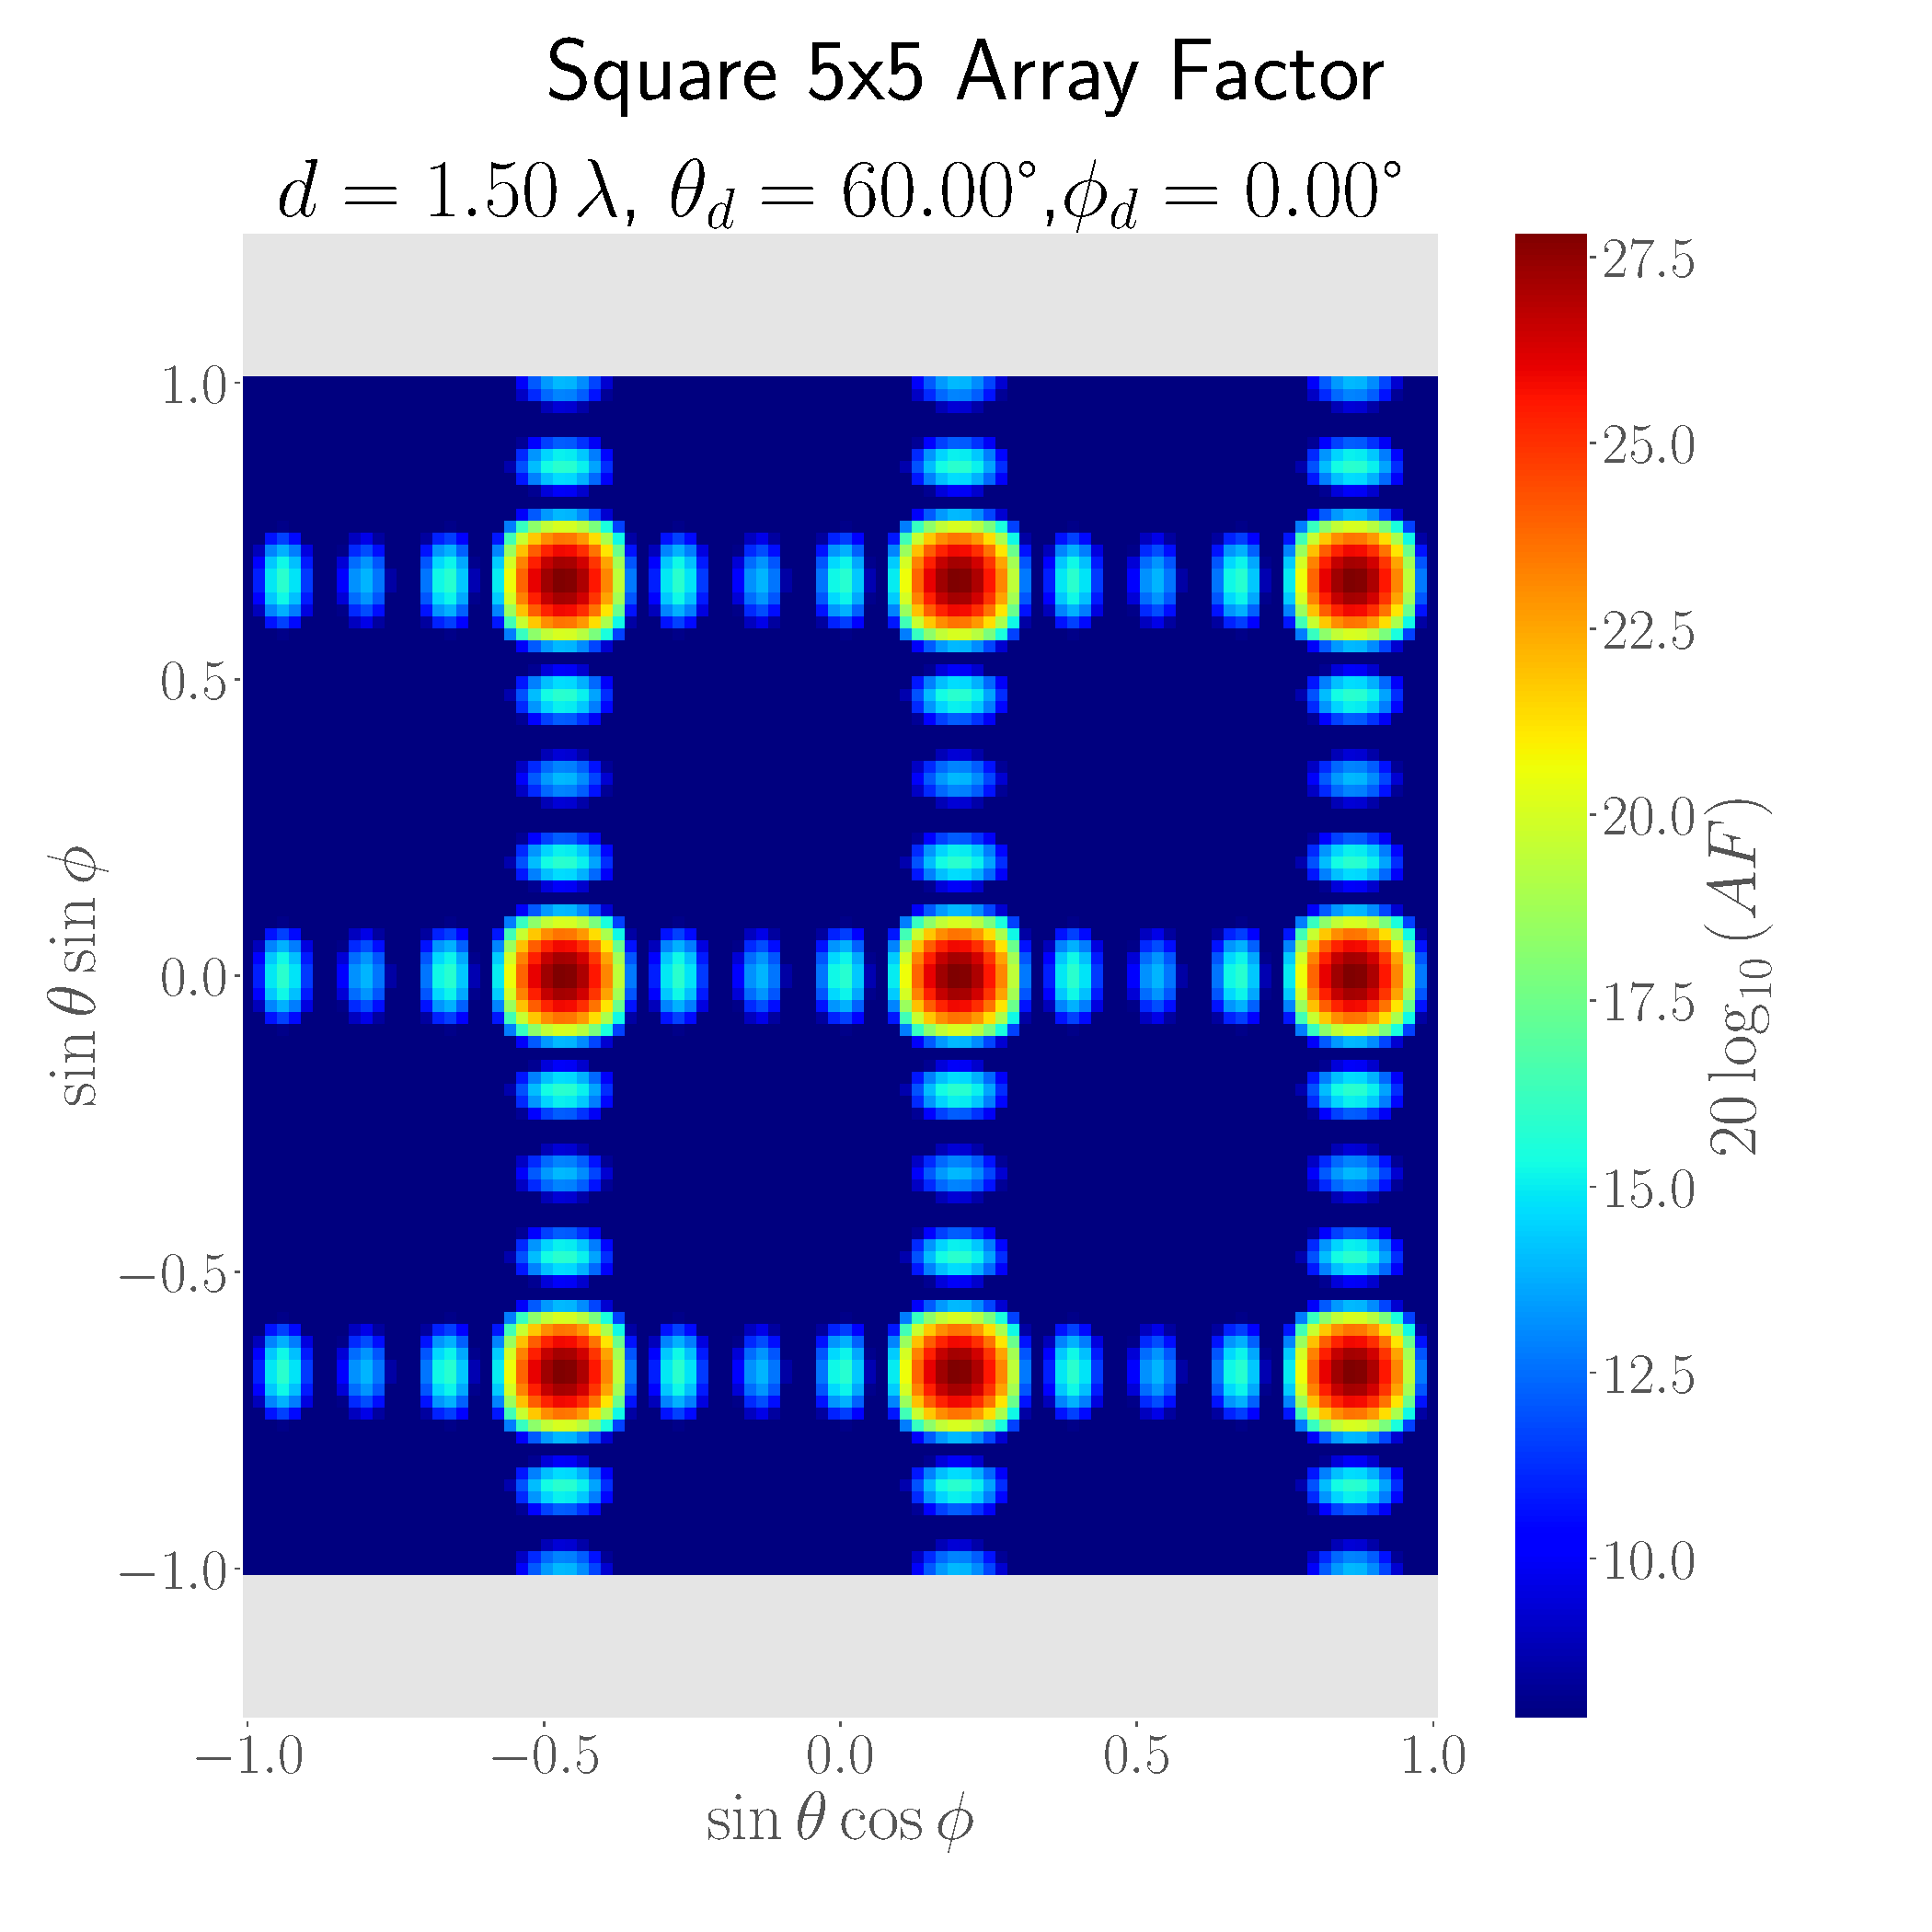
\includegraphics[width=\textwidth]{graphics/task_1/square-1.50-lambda-60.00-theta-0.00-phi-radpat.pdf}
    \caption{Square 5x5 off-vertically steered radiation pattern for $1.5\lambda$ spacing.}\label{fig:rad-square-1.5-60}
   \end{minipage}
\end{figure}



In the cases of figure \ref{fig:rad-square-1.0-0} and \ref{fig:rad-square-1.0-60}, the grating lobes become even more apparent. Although, technically the corner ones do not count since they lie beyond the array horizon. In this case and, also with $1.5\,\lambda$, spacing, you cannot distinguish the pattern resulting from the (wanted) $60\,\si{\degree}$ steering angle from a smaller one (e.g. $10\,\si{\degree}$), leading to unwanted ambiguities.



\subsection{Phase Distribution}

\begin{figure}[H]
  \begin{minipage}[t]{0.45\textwidth}
    \centering
    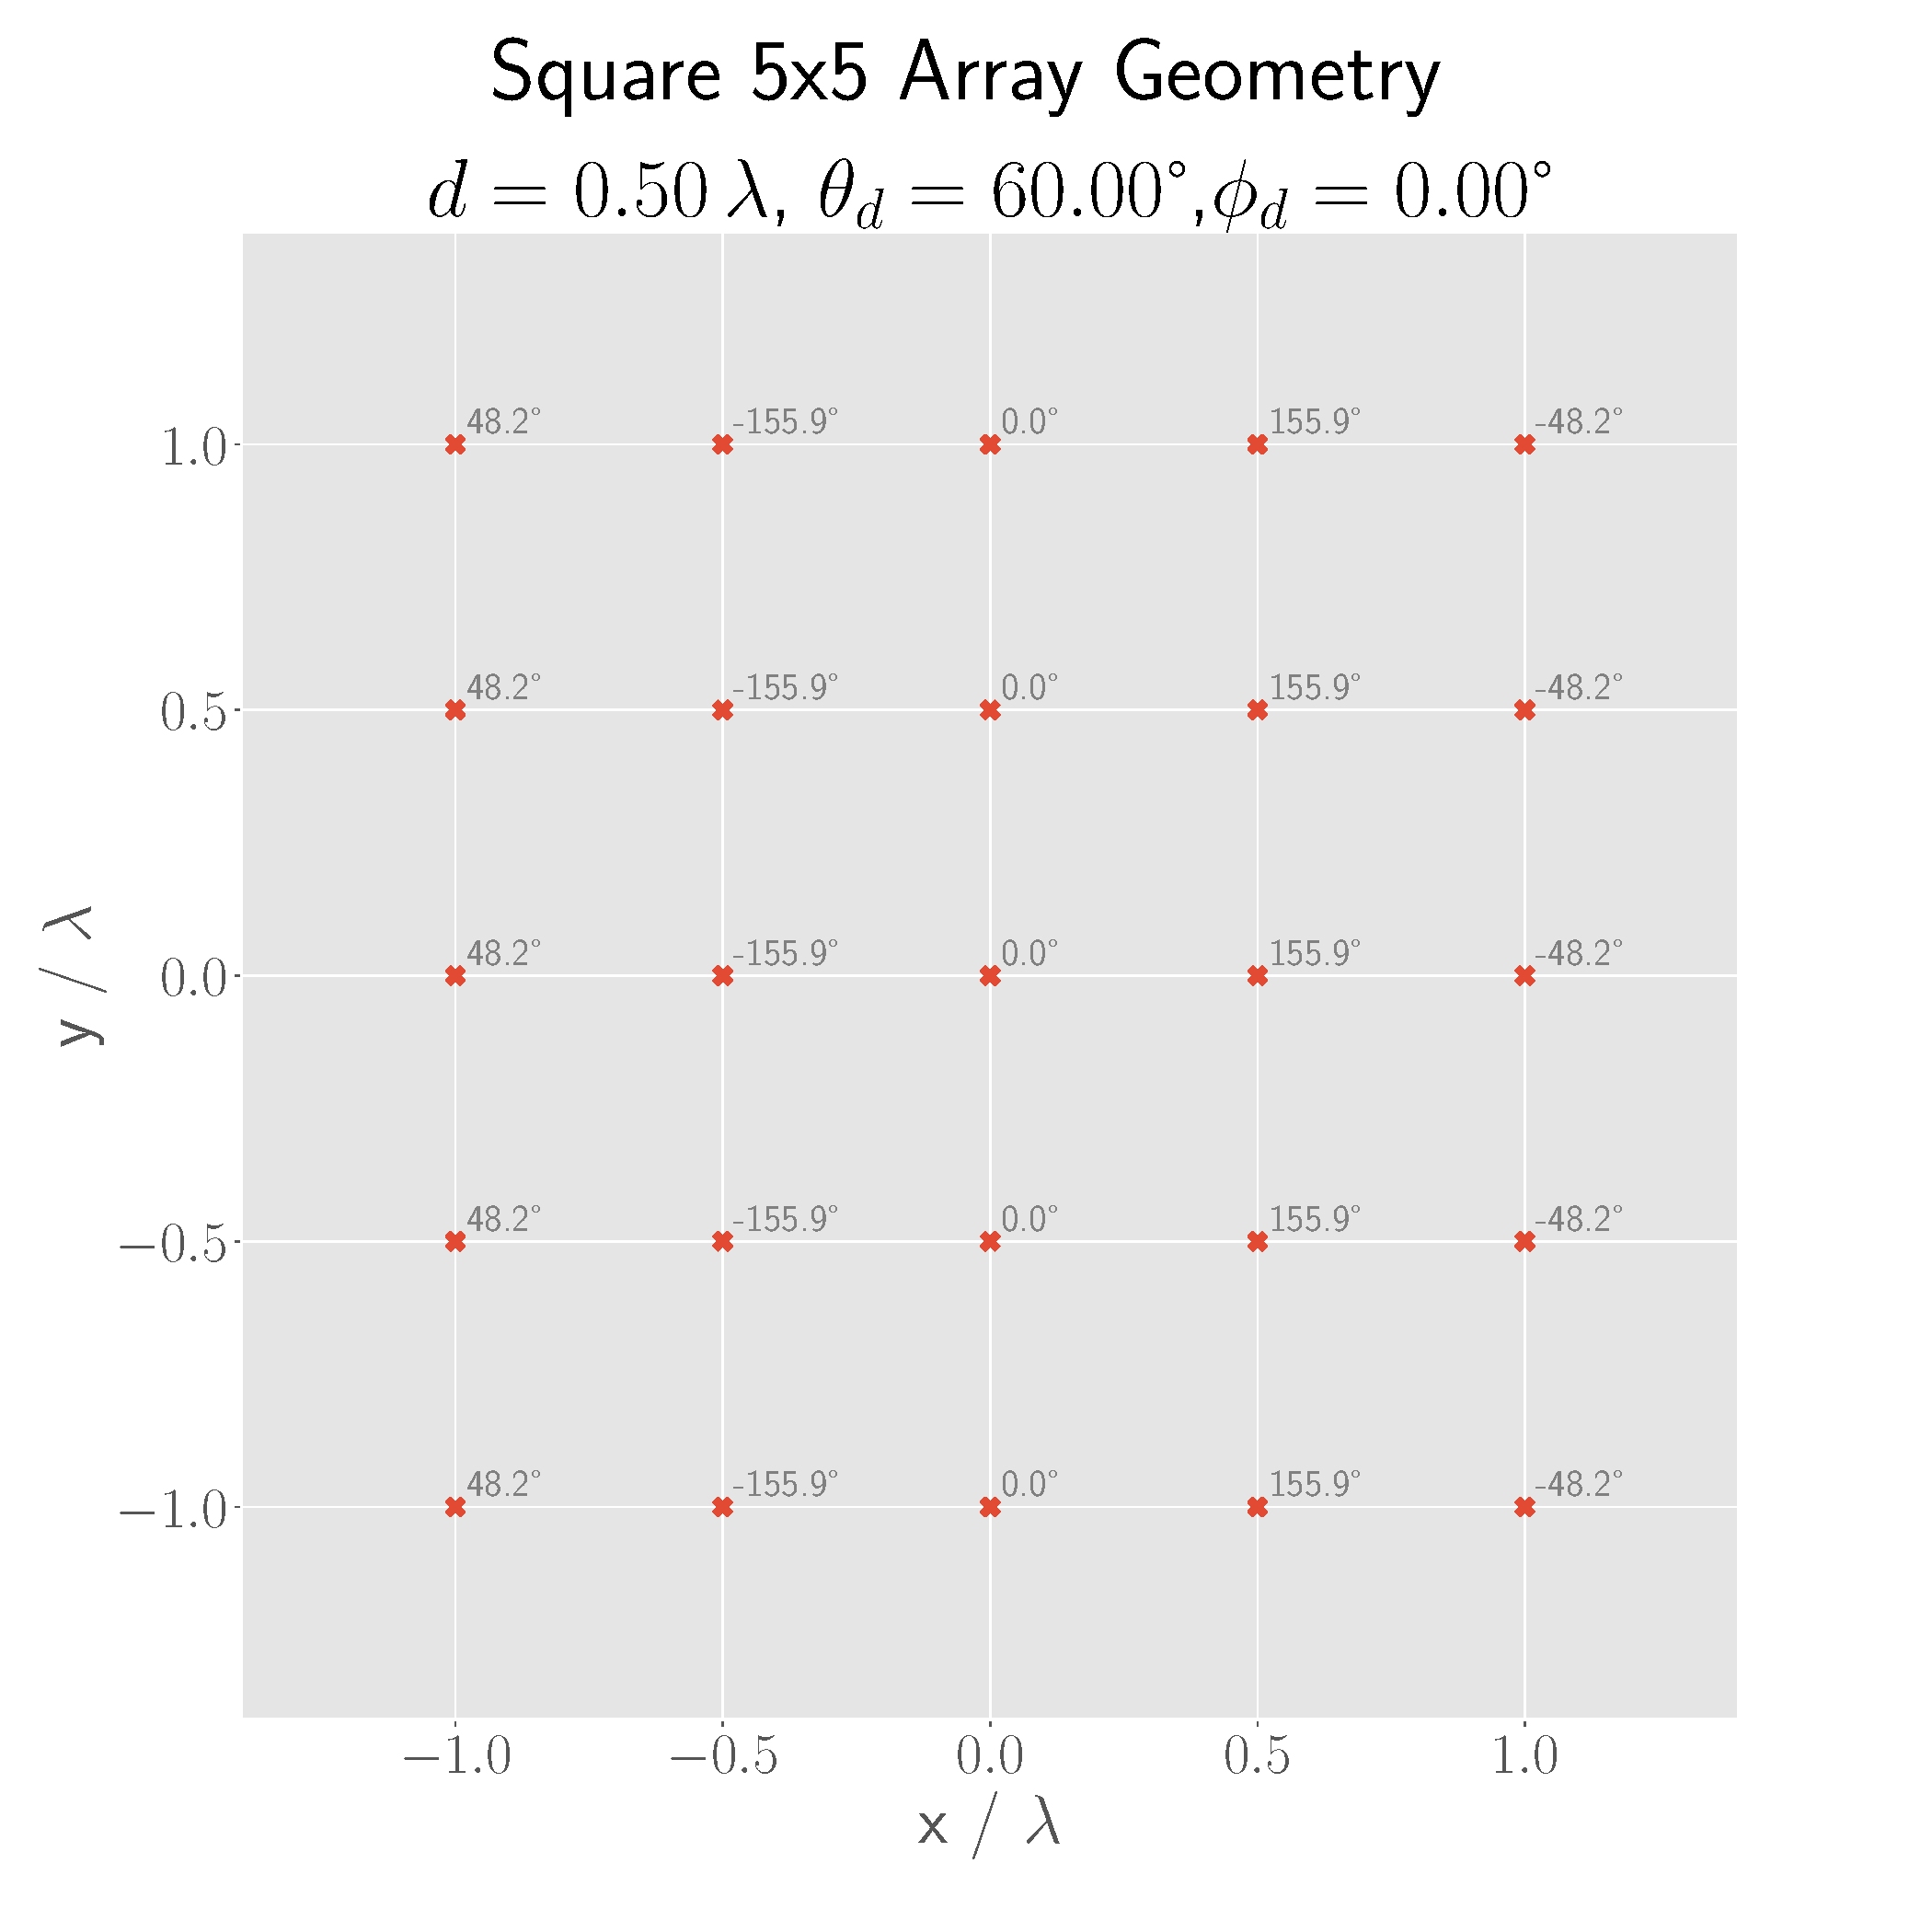
\includegraphics[width=\textwidth]{graphics/task_2/square-0.50-lambda-60.00-theta-0.00-phi-geometry.pdf}
    \caption{Square 5x5 Geometry with steering phases for $0.5\lambda$ spacing.}\label{fig:phase1}
  \end{minipage}\hfill
  \begin{minipage}[t]{0.45\textwidth}
    \centering
    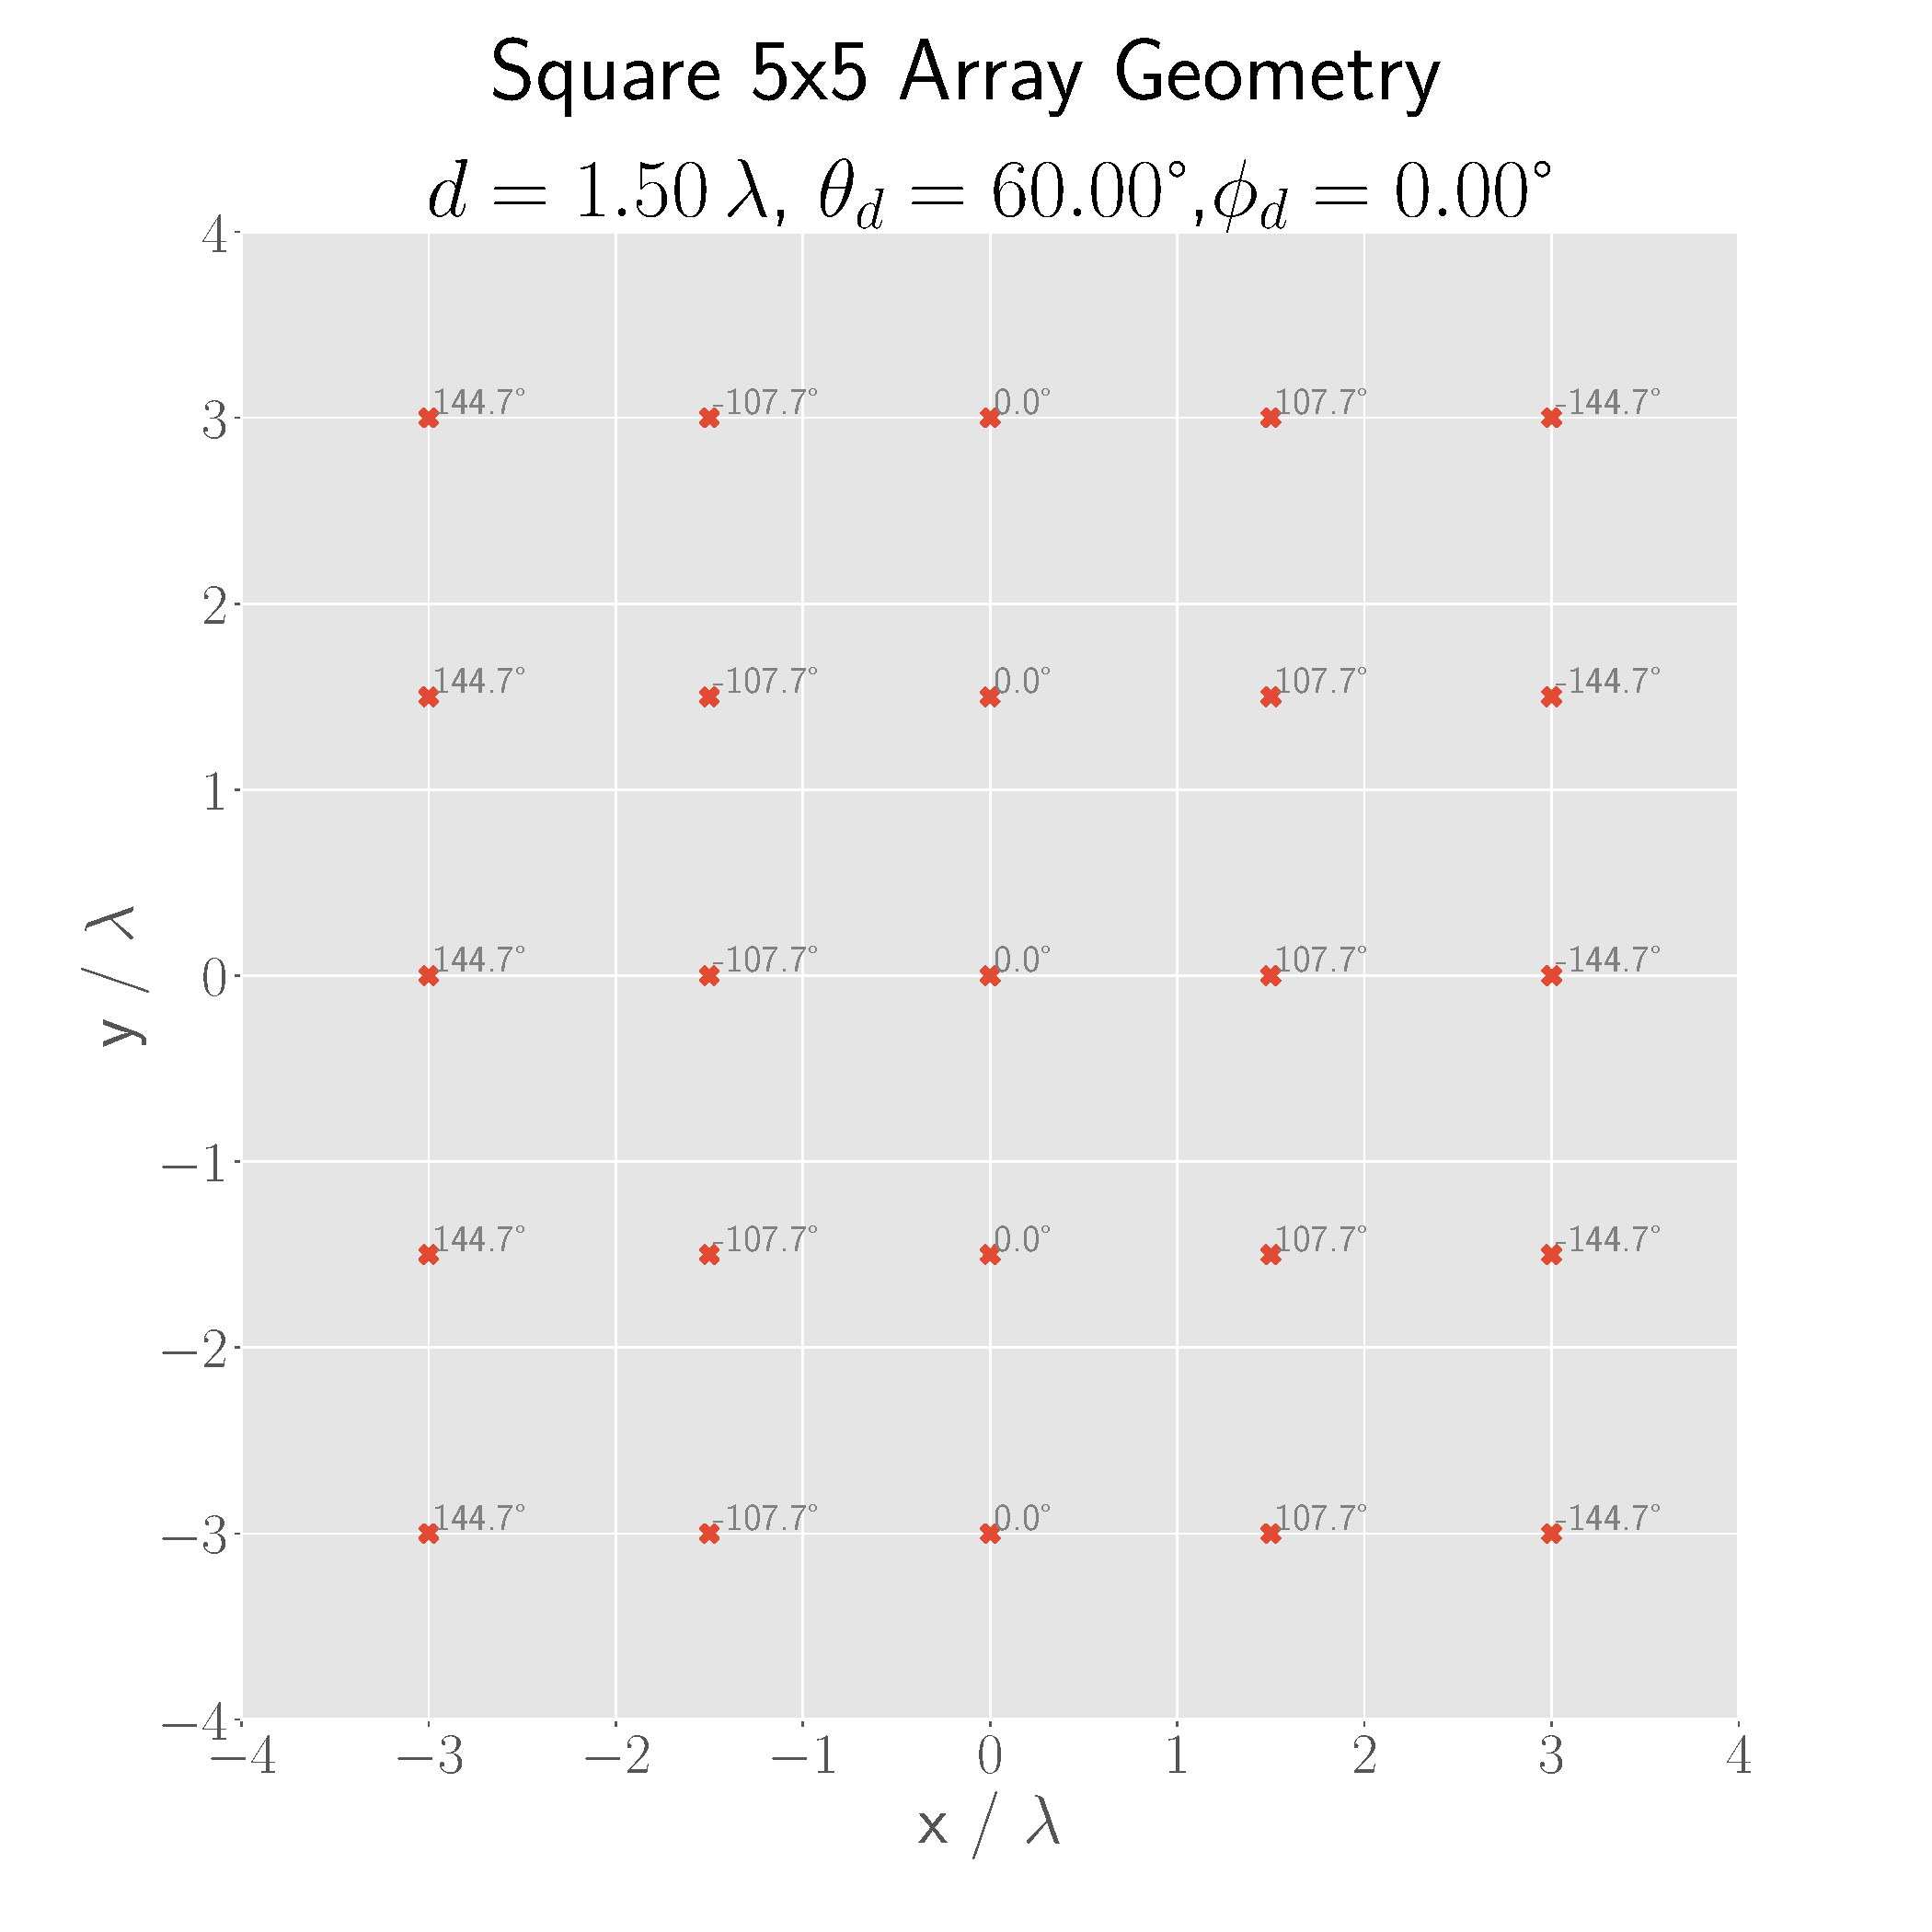
\includegraphics[width=\textwidth]{graphics/task_2/square-1.50-lambda-60.00-theta-0.00-phi-geometry.pdf}
    \caption{Square 5x5 Geometry with steering phases for $1.5\lambda$ spacing.}\label{fig:phase2}
   \end{minipage}
\end{figure}


In figures \ref{fig:phase1} and \ref{fig:phase2}, the array geometries along with the individual steering phases are shown for a target position of $\theta_{d}=60\,\si{\degree}, \phi_{d}=0\,\si{\degree}$. You can see that the phases are constant along the columns since any incident wave from a far-away target will have the same time of arrival for these antennas. Comparing the different spacings, the angle differences in the $d=1.5\lambda$ case are greater, which makes sense since their spacing is larger which results in more time lag.

